
\clearpage
\phantomsection
\addcontentsline{toc}{chapter}{CHƯƠNG 2: THIẾT KẾ QUAN NIỆM (ERD/EER)}
{\LARGE\bfseries CHƯƠNG 2: THIẾT KẾ QUAN NIỆM (ERD/EER)}\par\vspace{1em}

Chương này áp dụng phương pháp luận 6 bước của Chương 2 (khoanh phạm vi → lập từ điển nghiệp vụ → chọn ứng viên thực thể → rút quy tắc nghiệp vụ → xác định bản số → kiểm chứng bằng dữ liệu mẫu) cho nhóm lõi của FamilyConnect: Người dùng, Gia đình, Gia phả, Cộng đồng, Sự kiện.

\phantomsection
\addcontentsline{toc}{section}{2.1. Xác định thực thể}
{\Large\bfseries 2.1. Xác định thực thể}\par\vspace{0.7em}

\begin{longtable}{|p{0.3\textwidth}|p{0.3\textwidth}|p{0.3\textwidth}|}
\hline
\textbf{Thực thể} & \textbf{Loại} & \textbf{Lý do chọn làm thực thể } \\ \hline
\endfirsthead
\hline
\textbf{Thực thể} & \textbf{Loại} & \textbf{Lý do chọn làm thực thể } \\ \hline
\endhead
NGUOI\_DUNG (Users) & Mạnh & Có vòng đời độc lập (đăng ký/khóa tài khoản), nhiều thuộc tính riêng, tham gia nhiều mối kết hợp (viết bài, tham gia sự kiện...). \\ \hline
GIA\_DINH (Families) & Mạnh & Đối tượng gốc, cần tra cứu/thống kê riêng, nhiều dòng dữ liệu cụ thể. \\ \hline
CHI\_NHANH (Branches) & Mạnh, tự tham chiếu & Cần lưu lâu dài, có phân cấp cha–con trong cùng dòng họ. \\ \hline
THANH\_VIEN (FamilyMembers) & Mạnh & Trung tâm gia phả; có thể tồn tại độc lập với NGUOI\_DUNG (thành viên đã mất hoặc chưa có tài khoản). \\ \hline
BAI\_DANG (Posts) & Mạnh & Có vòng đời riêng (tạo/sửa/ghim), nhiều thuộc tính mô tả. \\ \hline
BINH\_LUAN (Comments) & Mạnh, tự tham chiếu & Cần tra cứu riêng, có quan hệ trả lời đệ quy. \\ \hline
SU\_KIEN (Events) & Mạnh & Nhiều thuộc tính riêng (thời gian, địa điểm), tham gia mối kết hợp M:N với thành viên. \\ \hline
NHAC\_SU\_KIEN (EventReminders) & Yếu & Không có ý nghĩa nếu tách khỏi SU\_KIEN — xem mục 2.3. \\ \hline
\end{longtable}


\phantomsection
\addcontentsline{toc}{section}{2.2. Phân loại thuộc tính tiêu biểu}
{\Large\bfseries 2.2. Phân loại thuộc tính tiêu biểu}\par\vspace{0.7em}

\begin{longtable}{|p{0.3\textwidth}|p{0.3\textwidth}|p{0.3\textwidth}|}
\hline
\textbf{Thuộc tính} & \textbf{Loại (theo Chương 2)} & \textbf{Diễn giải} \\ \hline
\endfirsthead
\hline
\textbf{Thuộc tính} & \textbf{Loại (theo Chương 2)} & \textbf{Diễn giải} \\ \hline
\endhead
THANH\_VIEN.hoTen & Đơn & Giá trị nguyên tử, không cần tách. \\ \hline
THANH\_VIEN.diaChi (nếu mở rộng) & Phức hợp & Có thể tách soNha/quan/thanhPho nếu cần thống kê theo khu vực. \\ \hline
NGUOI\_DUNG.soDienThoai (mở rộng đa số) & Đa trị & Một người dùng có thể có nhiều số liên hệ — tách bảng riêng nếu nghiệp vụ yêu cầu. \\ \hline
THANH\_VIEN.doTuoi (tuổi) & Dẫn xuất & Tính từ dateOfBirth — không lưu trực tiếp để tránh mâu thuẫn dữ liệu theo thời gian. \\ \hline
THANH\_VIEN.isAlive & Đơn (cờ trạng thái) & Suy ra được một phần từ dateOfDeath nhưng lưu trực tiếp để truy vấn nhanh mà không phải tính lại. \\ \hline
\end{longtable}


\phantomsection
\addcontentsline{toc}{section}{2.3. Mối kết hợp, bản số và mức tham gia}
{\Large\bfseries 2.3. Mối kết hợp, bản số và mức tham gia}\par\vspace{0.7em}

Sơ đồ ERD theo ký pháp Chen (Hình 2.1) trình bày các thực thể, mối kết hợp (hình thoi) và bản số hai phía cho nhóm lõi. Bảng 2.3 liệt kê đầy đủ mối kết hợp kèm bản số và mức tham gia tối thiểu/tối đa.

\begin{figure}[H]
\centering
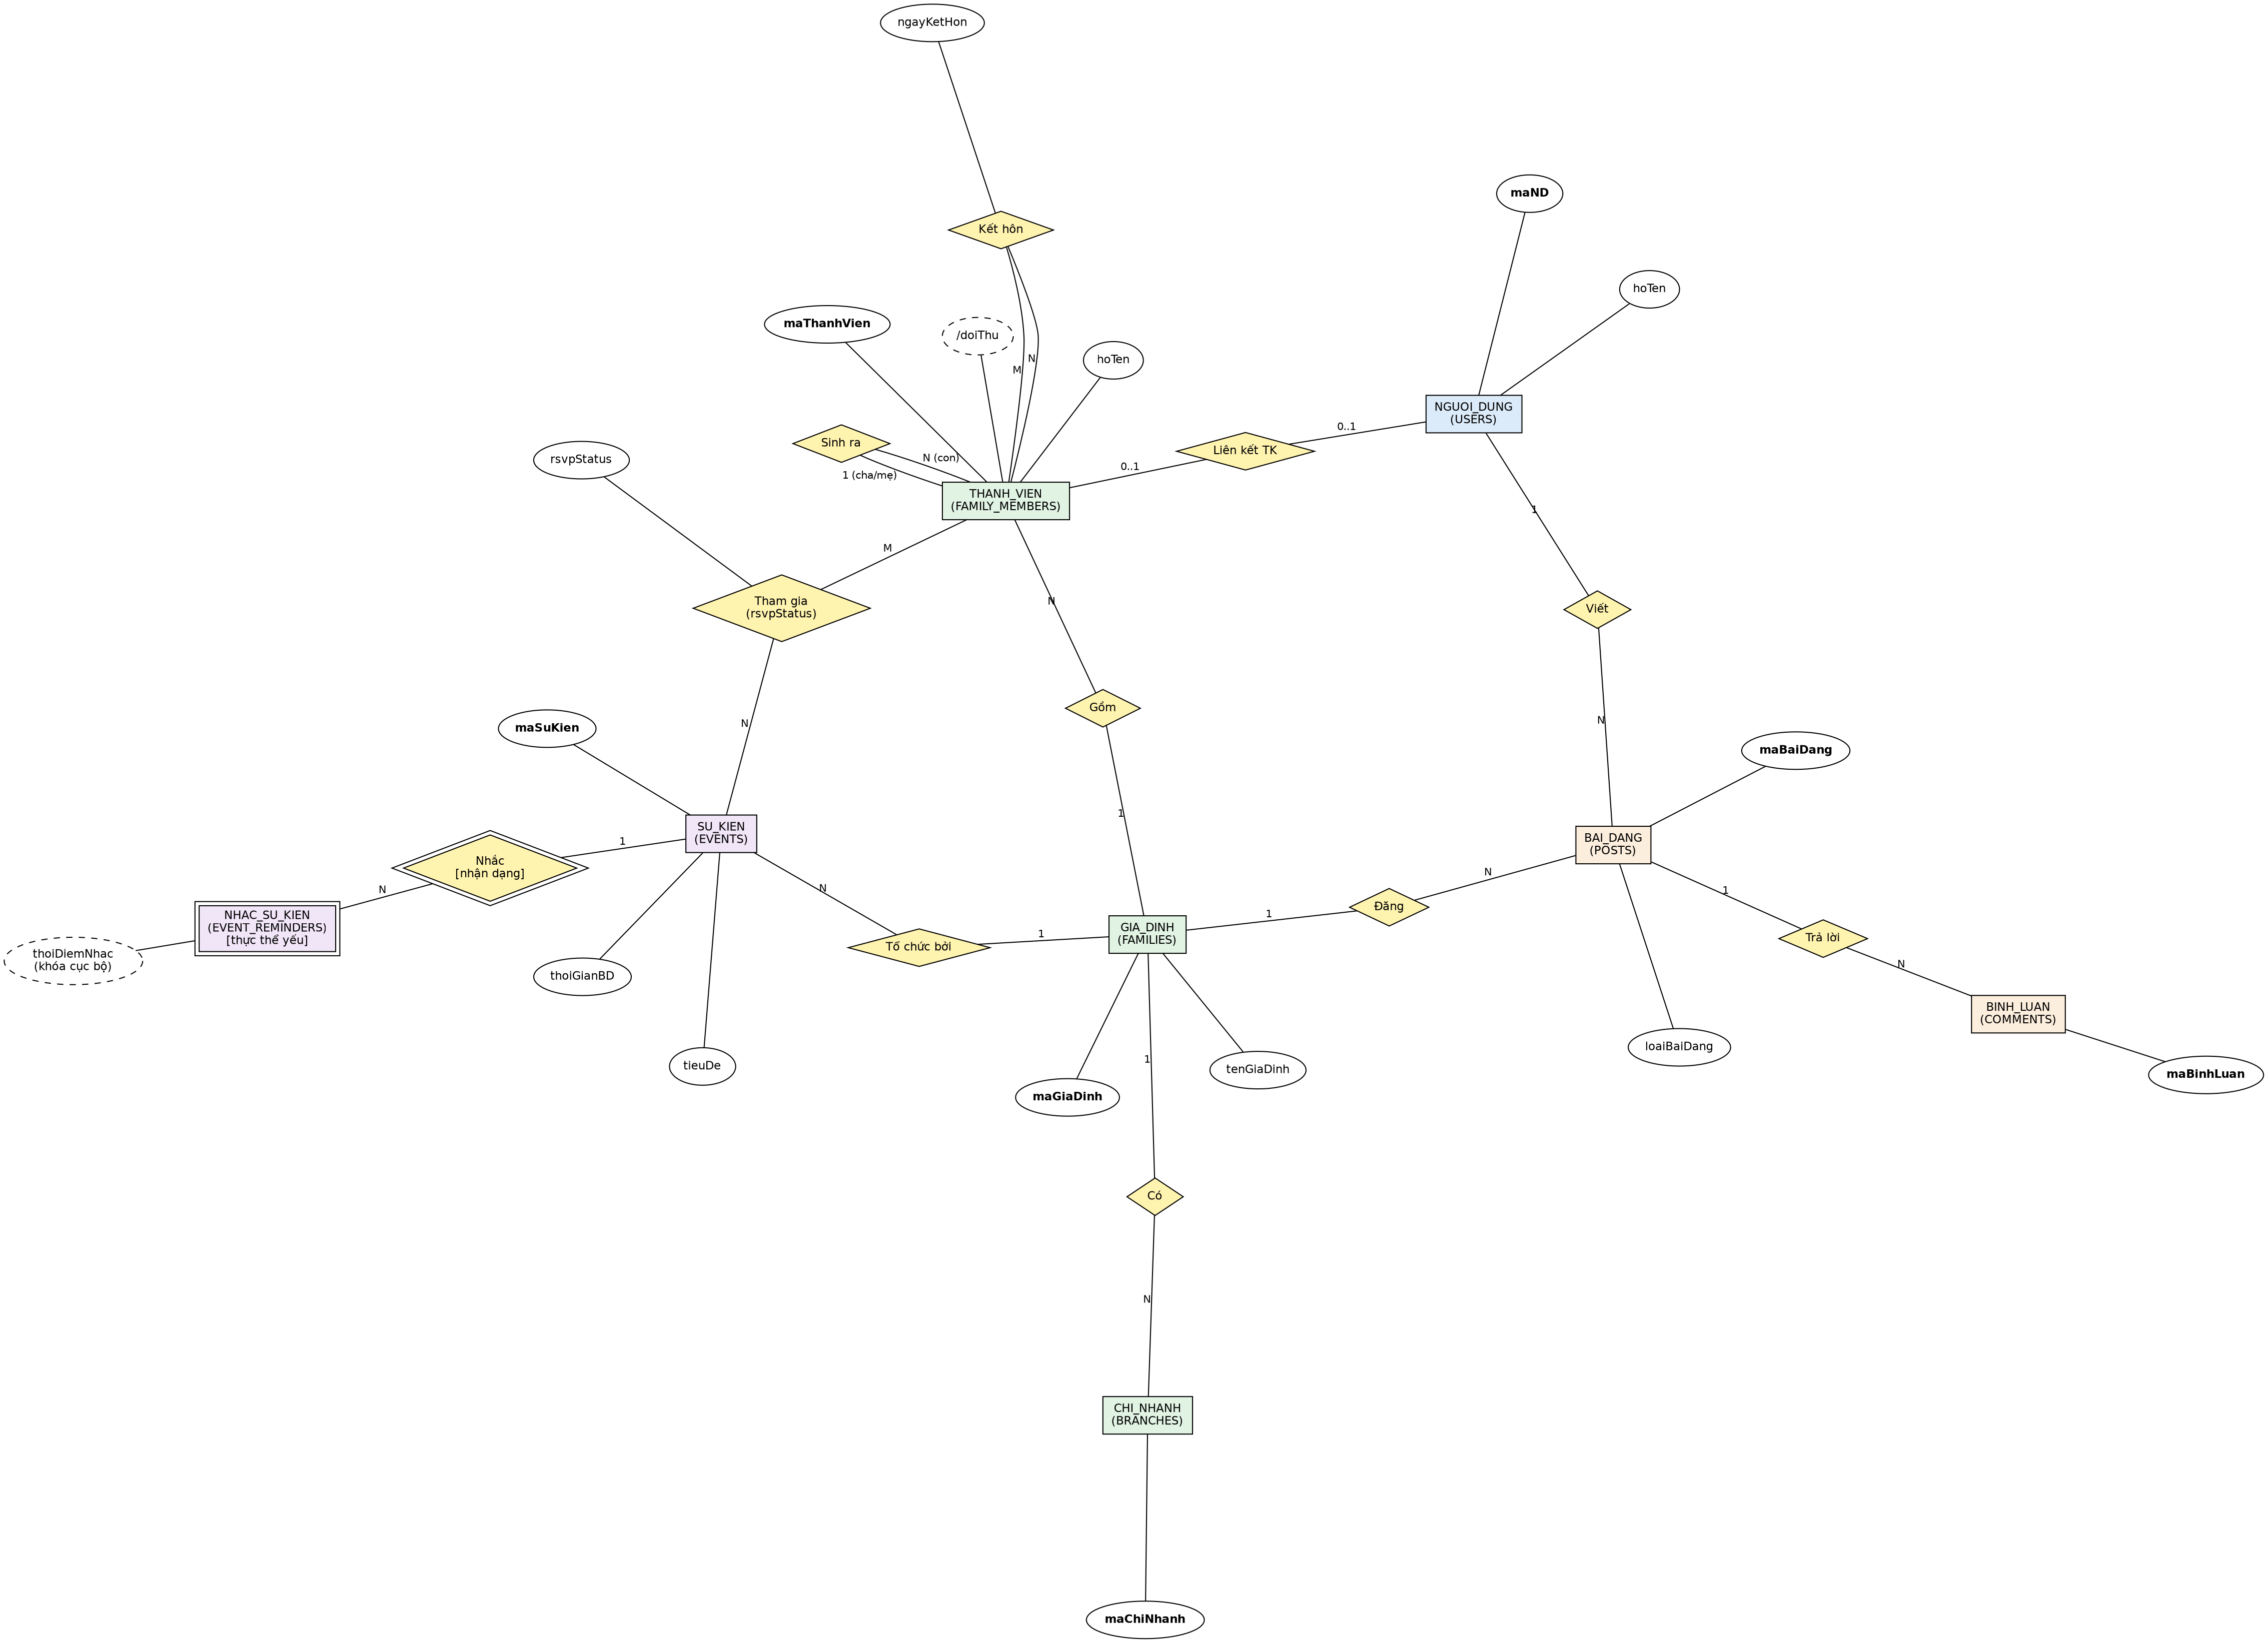
\includegraphics[width=0.95\textwidth]{images/image1.png}
\caption{\emph{Hình 2.1. Sơ đồ ERD ký pháp Chen — nhóm lõi Người dùng, Gia phả, Cộng đồng, Sự kiện của FamilyConnect}}
\end{figure}

\begin{longtable}{|p{0.225\textwidth}|p{0.225\textwidth}|p{0.225\textwidth}|p{0.225\textwidth}|}
\hline
\textbf{Mối kết hợp} & \textbf{Bản số} & \textbf{Mức tham gia} & \textbf{Ghi chú} \\ \hline
\endfirsthead
\hline
\textbf{Mối kết hợp} & \textbf{Bản số} & \textbf{Mức tham gia} & \textbf{Ghi chú} \\ \hline
\endhead
GIA\_DINH – Có – CHI\_NHANH & 1:N & GIA\_DINH: tùy chọn (0..*); CHI\_NHANH: bắt buộc (1) & Chi nhánh không tồn tại nếu không có dòng họ \\ \hline
GIA\_DINH – Gồm – THANH\_VIEN & 1:N & THANH\_VIEN bắt buộc (1) & Mỗi thành viên gia phả thuộc đúng một dòng họ \\ \hline
NGUOI\_DUNG – Liên kết TK – THANH\_VIEN & 0..1 : 0..1 & Cả hai phía tùy chọn & Thành viên có thể chưa có tài khoản; tài khoản có thể chưa liên kết gia phả \\ \hline
THANH\_VIEN – Sinh ra – THANH\_VIEN (đệ quy) & N:2 (dạng M:N bị giới hạn) & Phía cha/mẹ: tùy chọn, không giới hạn (0..*); phía con bắt buộc có tối đa 2 cha/mẹ (ràng buộc nghiệp vụ) & Không phải 1:N thuần túy: một con có thể có tối đa 2 cha/mẹ nên cần bảng trung gian ParentChildRelationships (giống ánh xạ M:N), khác với 1:N chuẩn (chỉ cần FK trực tiếp trên bảng con); giới hạn "tối đa 2" được ép buộc thêm bằng CHECK/trigger ở mức vật lý \\ \hline
THANH\_VIEN – Kết hôn – THANH\_VIEN (đệ quy) & M:N & Tùy chọn cả hai phía & Có thuộc tính riêng: ngayKetHon, trạng thái — trở thành thực thể kết hợp MARRIAGES \\ \hline
GIA\_DINH – Đăng – BAI\_DANG & 1:N & BAI\_DANG bắt buộc (1) & Bài đăng luôn thuộc một dòng họ cụ thể; xóa dòng họ kéo theo xóa toàn bộ bài đăng liên quan \\ \hline
NGUOI\_DUNG – Viết – BAI\_DANG & 1:N & BAI\_DANG bắt buộc (1) & Tác giả bài đăng là người dùng đã liên kết tài khoản, không phải mọi thành viên gia phả \\ \hline
BAI\_DANG – Trả lời – BINH\_LUAN & 1:N & BINH\_LUAN bắt buộc (1) & BINH\_LUAN cũng tự tham chiếu (reply lồng nhau) \\ \hline
GIA\_DINH – Tổ chức bởi – SU\_KIEN & 1:N & SU\_KIEN bắt buộc (1) & Sự kiện luôn gắn với một dòng họ tổ chức, dùng để lọc/phân quyền hiển thị \\ \hline
THANH\_VIEN – Tham gia – SU\_KIEN & M:N & Tùy chọn cả hai phía & Có thuộc tính riêng rsvpStatus → thực thể kết hợp EVENT\_PARTICIPANTS \\ \hline
SU\_KIEN – Nhắc – NHAC\_SU\_KIEN & 1:N, mối kết hợp nhận dạng & NHAC\_SU\_KIEN tham gia toàn phần, bắt buộc (1) & Mối kết hợp nhận dạng của thực thể yếu — xem mục 2.4 \\ \hline
\end{longtable}


\phantomsection
\addcontentsline{toc}{section}{2.4. Thực thể yếu}
{\Large\bfseries 2.4. Thực thể yếu}\par\vspace{0.7em}

Áp dụng tiêu chí ("thực thể yếu không đủ thuộc tính để định danh độc lập, cần thực thể chủ để có ý nghĩa"), FamilyConnect có ba trường hợp phụ thuộc cần xem xét, trong đó hai trường hợp là thực thể yếu đúng nghĩa (USER\_PROFILES, EVENT\_REMINDERS) và một trường hợp cần xếp lại thành thực thể mạnh có phụ thuộc tồn tại (xem phân tích MEMBER\_VERIFICATIONS bên dưới):

\begin{longtable}{|p{0.3\textwidth}|p{0.3\textwidth}|p{0.3\textwidth}|}
\hline
\textbf{Thực thể yếu} & \textbf{Thực thể chủ / khóa cục bộ} & \textbf{Lý do \& khóa chính sau khi ánh xạ} \\ \hline
\endfirsthead
\hline
\textbf{Thực thể yếu} & \textbf{Thực thể chủ / khóa cục bộ} & \textbf{Lý do \& khóa chính sau khi ánh xạ} \\ \hline
\endhead
USER\_PROFILES & Users / khóa cục bộ = chính UserId (chia sẻ khóa) & Hồ sơ mở rộng không có ý nghĩa nếu tài khoản không tồn tại. Khóa chính = UserId (PK/FK), quan hệ nhận dạng 1:1. \\ \hline
MEMBER\_VERIFICATIONS (*) & FamilyMembers / phụ thuộc tồn tại (existence dependency), không dùng khóa cục bộ ghép & (*) Xét lại theo lý thuyết Chương 2: khóa chính thực tế là VerificationId (UUID) đứng độc lập, không phải khóa ghép (MemberId + khóa cục bộ) như định nghĩa chuẩn của thực thể yếu. FK MemberId bắt buộc + ON DELETE CASCADE chỉ thể hiện phụ thuộc tồn tại, không phải phụ thuộc nhận dạng. Do đó MEMBER\_VERIFICATIONS nên được xếp là thực thể mạnh (dùng khóa thay thế) có ràng buộc tồn tại vào FamilyMembers, khác với EVENT\_REMINDERS bên dưới — trường hợp mới đúng là thực thể yếu (khóa ghép EventId + RemindAt). \\ \hline
EVENT\_REMINDERS & Events / khóa cục bộ = RemindAt & Một lời nhắc chỉ có nghĩa trong ngữ cảnh một sự kiện; RemindAt có thể trùng giữa các sự kiện khác nhau. Khóa chính = (EventId, RemindAt) — khóa chủ + khóa cục bộ, đúng Thuật toán 2.3 (Weak Entity Mapping). \\ \hline
\end{longtable}


\phantomsection
\addcontentsline{toc}{section}{2.5. EER: chuyên biệt hóa vai trò người dùng}
{\Large\bfseries 2.5. EER: chuyên biệt hóa vai trò người dùng}\par\vspace{0.7em}

Khi một thực thể có các nhóm hành vi khác nhau, có thể mô hình bằng chuyên biệt hóa (specialization) với ràng buộc rời nhau/chồng lấp (disjoint/overlap) và toàn phần/từng phần (complete/incomplete). Với FamilyConnect, NGUOI\_DUNG có thể giữ nhiều vai trò cùng lúc trong các dòng họ khác nhau (một người có thể vừa là FamilyAdmin của dòng họ A vừa là Member của dòng họ B), và không phải người dùng nào cũng có vai trò quản trị.

Đây là ràng buộc \{overlapping, incomplete\}: một người dùng có thể thuộc nhiều lớp vai trò con hoặc không thuộc lớp con nào ngoài vai trò Member mặc định. Theo hai chiến lược ánh xạ EER của Chương 2 ("cha–con" tạo bảng riêng cho từng lớp con, hoặc "một bảng" gộp chung có cột phân loại):

\begin{itemize}
\item Chiến lược cha–con (từng bảng con FamilyAdmin, Moderator...) sẽ tạo nhiều bảng con cho một quan hệ chồng lấp — không phù hợp vì một người dùng có thể thuộc nhiều lớp con cùng lúc.
\item Chiến lược một bảng gộp (thêm cột loaiVaiTro) không biểu diễn được việc một người có nhiều vai trò đồng thời và không biểu diễn được phạm vi 'theo từng dòng họ'.
\item Do đó, đồ án chọn phương án thứ ba — phổ biến khi quan hệ là \{overlap, incomplete\} và có ngữ cảnh (theo dòng họ): dùng bảng trung gian n-n ROLES/USER\_ROLES(UserId, RoleId, FamilyId). Đây là cách hiện thực hóa quan hệ EER chồng lấp bằng mô hình quan hệ chuẩn, tương đương một 'bảng lớp con ảo' cho phép nhiều dòng.
\end{itemize}

Việc phân tích đánh đổi này thể hiện đúng tinh thần Chương 2: chọn chiến lược ánh xạ EER dựa trên ràng buộc rời nhau/chồng lấp và toàn phần/từng phần của bài toán thực tế, thay vì áp dụng máy móc một khuôn mẫu.

\phantomsection
\addcontentsline{toc}{section}{2.6. Sơ đồ ERD tổng thể toàn hệ thống (mức logic)}
{\Large\bfseries 2.6. Sơ đồ ERD tổng thể toàn hệ thống (mức logic)}\par\vspace{0.7em}

Sau khi áp dụng cùng phương pháp luận trên cho các nhóm chức năng còn lại (Danh bạ, Di sản, AI, Báo cáo, Quản trị), Hình 2.2 trình bày toàn bộ 33 thực thể/quan hệ và các mối kết hợp khóa ngoại, làm nền cho chương thiết kế logic.

\begin{figure}[H]
\centering
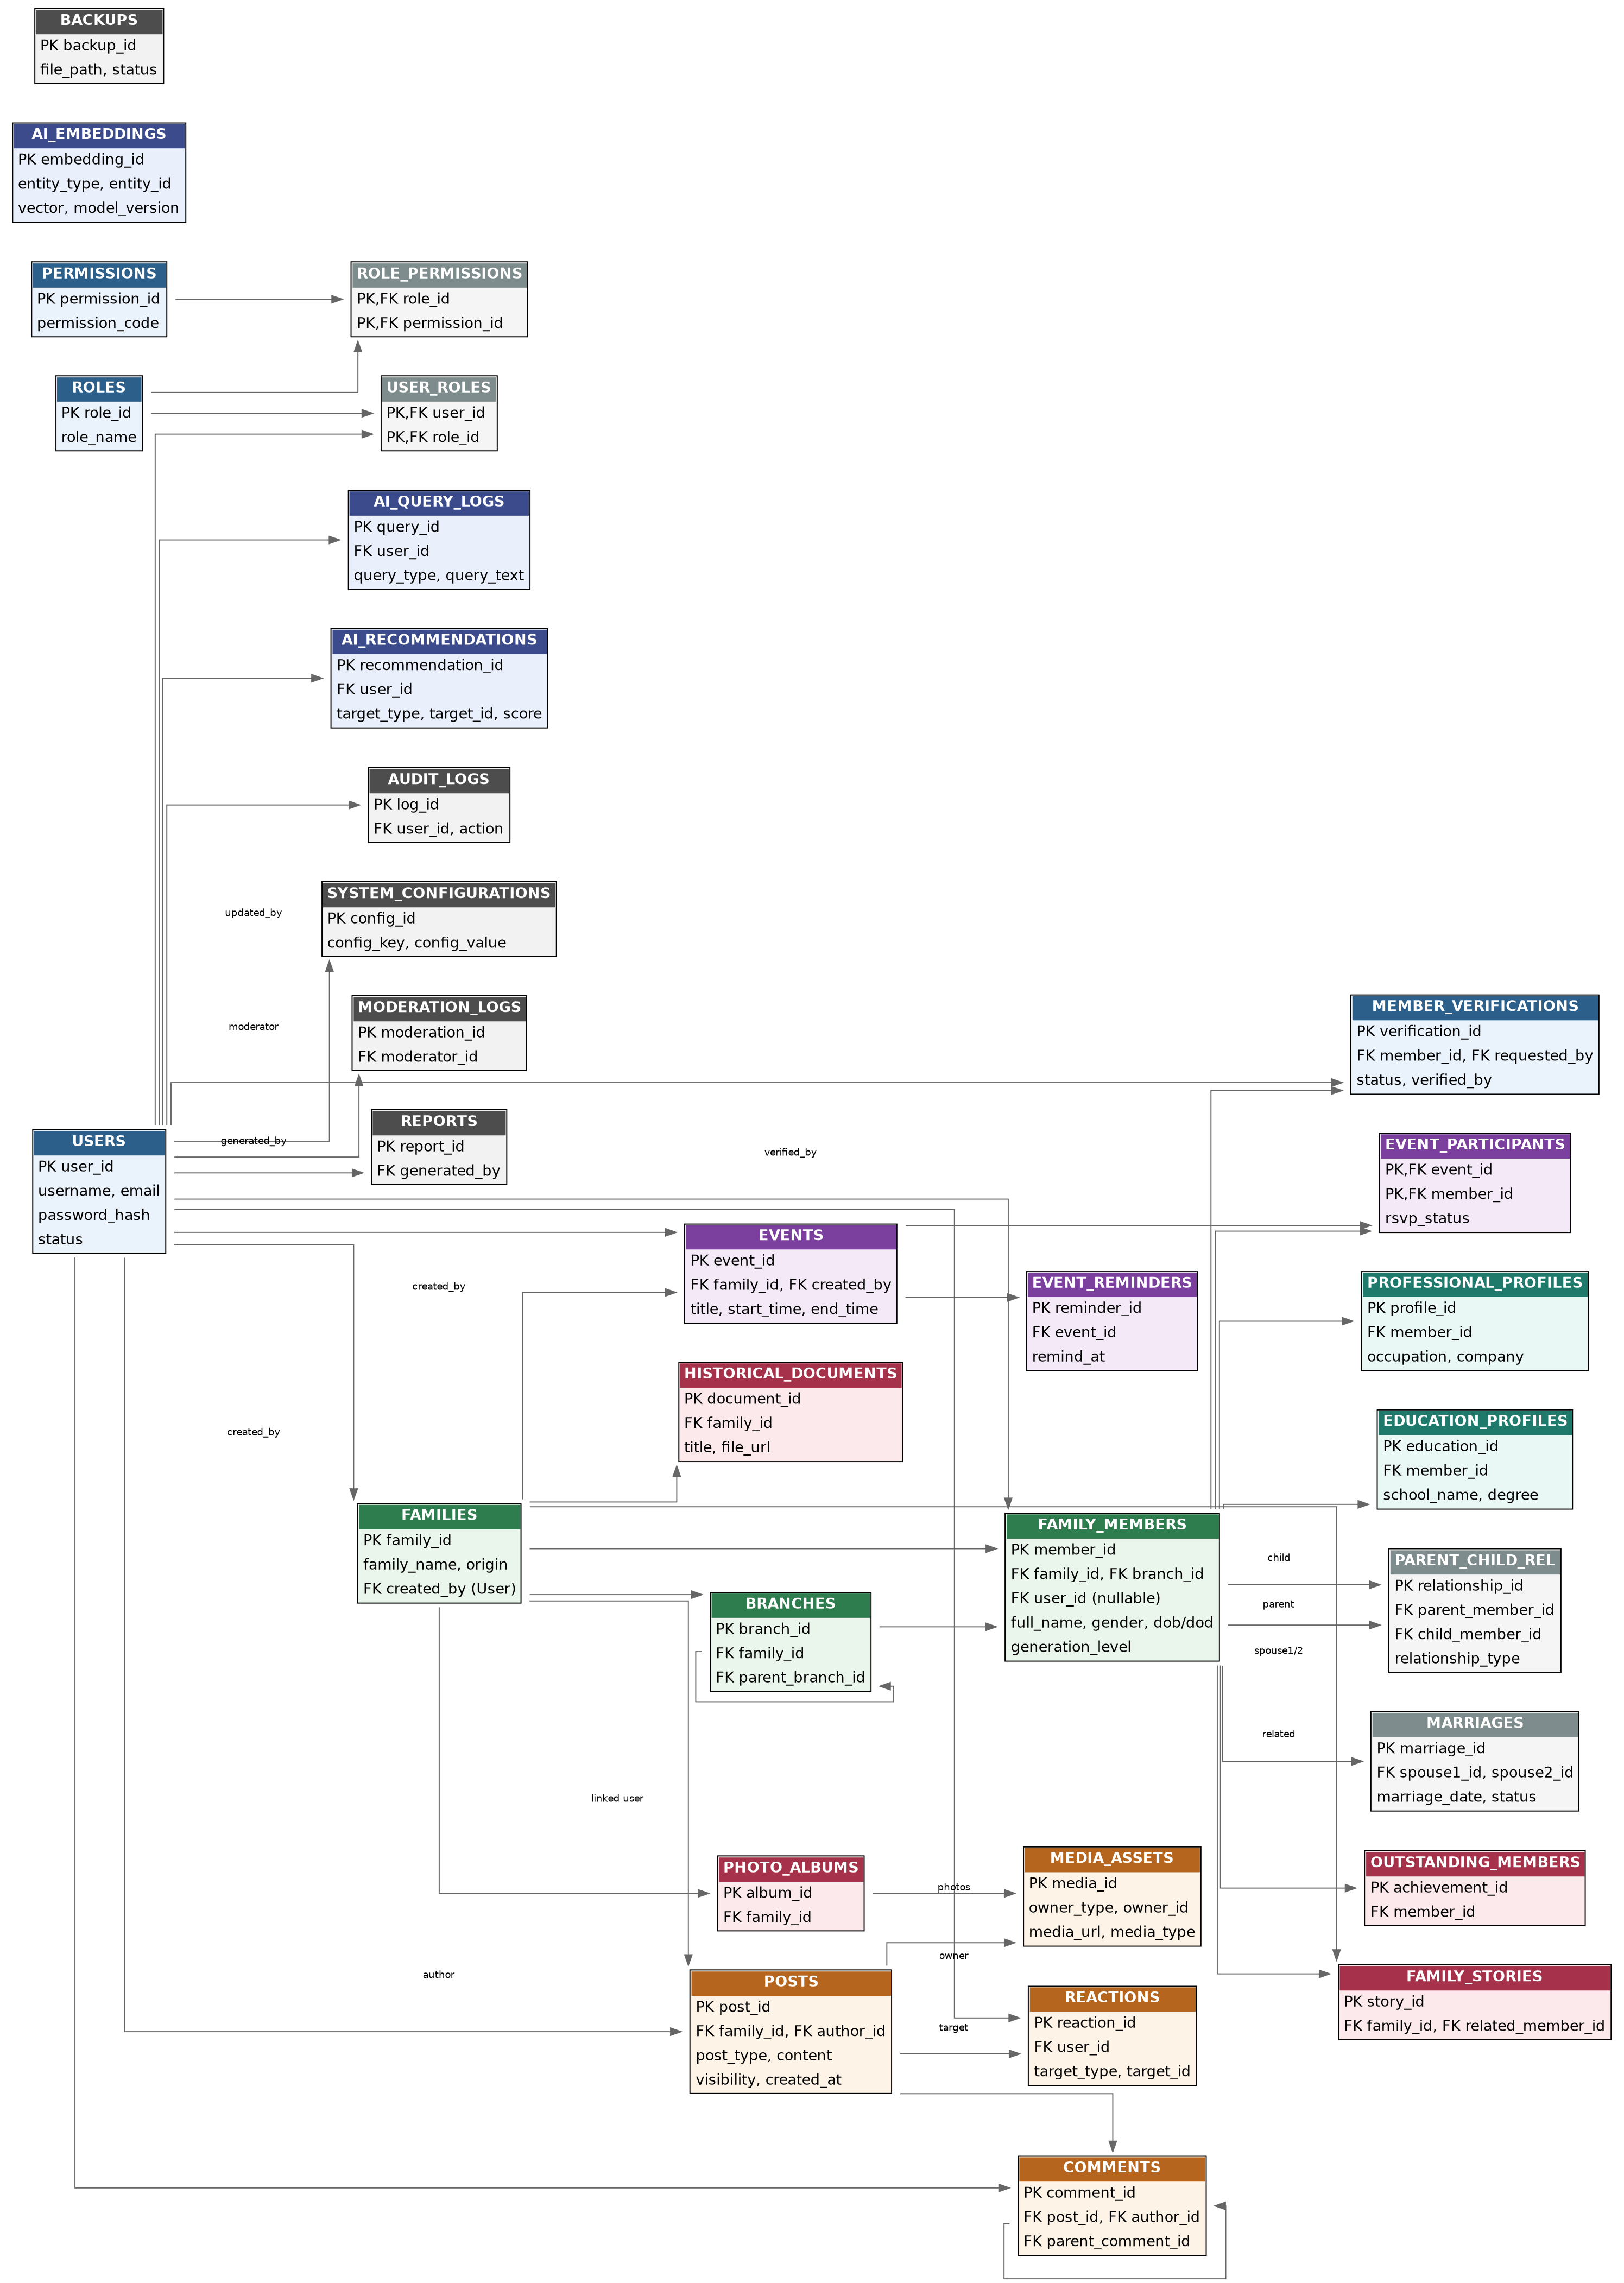
\includegraphics[width=0.95\textwidth]{images/image2.png}
\caption{\emph{Hình 2.2. Sơ đồ tổng thể các thực thể/quan hệ và khóa ngoại của FamilyConnect}}
\end{figure}